\documentclass[12pt]{article}
\usepackage{apacite,rotating,array,booktabs,ctable,graphicx,tabularx,amsfonts, amsmath, amsthm,url,multirow,verbatim}
\usepackage[top=1in,right=1in,left=1in,bottom=1in]{geometry}
\usepackage[T1]{fontenc}
\usepackage{cmbright}


\newcommand{\putbib}[1]{
\bibliographystyle{apacite}
\bibliography{./#1}
}	
\title{Model Selection by Testing Conjoint Checks}
\date{}

\begin{document}
\maketitle
\section{Results}
The model selection framework discussed in \citeA{torres2012}, specifically as it is laid out in Figure 4, was analyzed along the lines suggested in \citeA{domingue2013} (implemented as \citeNP{conjointchecks}). The distribution of the violations found are shown in Figure \ref{boxplots}.\footnote{what about adding 2pl, 3pl and other irt models to these?} For both unweigthed and weighted mean violations, the algorithm clearly distinguishes between the UNC and MON models on one hand and the IIO, DM, LCR, and RSH models on the other. Figure 4 of \citeA{torres2012} suggests a reason for why this might be so. The first two models, UNC and MON, do not impose invariant item ordering. All of the other models do. The distinction between MON and IIO is worth further consideration. MON imposes invariant person ordering while IIO imposes invariant item ordering. Although each imposes one type of single cancellation, neither requires both types. Why, then, does IIO fare so much better? This is simply a function of the fact that the means considered in Figure \ref{boxplots} were computed at the item level. {\bf NOTE: My thinking here has actually evolved. The mean of the item-level and person-level means across the tests will be, duh, the same. I think it actually has everything to do with the accuracy of item-level and person-level estimates. The latter are just total noise.}\footnote{A nice way of showing the fuzziness of the estimates might be to consider the true theta's gathered into each sum score and then look at the within versus between variance of true scores as grouped into sum scores. I did this at some point and it is quite provocative.}

The fact that the algorithm, which simultaneously checks for both forms of single cancellation as well as double cancellation, can not distinguish between the IIO, DM, LCR, and RSH models is surprising. Since LCR and RSH allow for quantitative structure, they should have fewer detected violations than the IIO and DM models which only allow for differences in order.\footnote{I have to admit to something. I have occasionally said something like: non-crossing item and person response curves are sufficient for quantity. But clearly this isn't true (consider DM). What am I missing?} The reason for this is subtle and will be demonstrated in the next section. In brief, checking for double cancellation, at least as it is suggested in \citeA{domingue2013}, requires so many ``fixes'' due to the total lack of ordering that can be assumed along minor diagonals that it effectively adds nothing above and beyond single cancellation to the stringency of the checks.

\begin{figure}
\centering
\caption{Boxplots showing distribution of violation means (unweighted and weighted) for the different models} \label{boxplots}
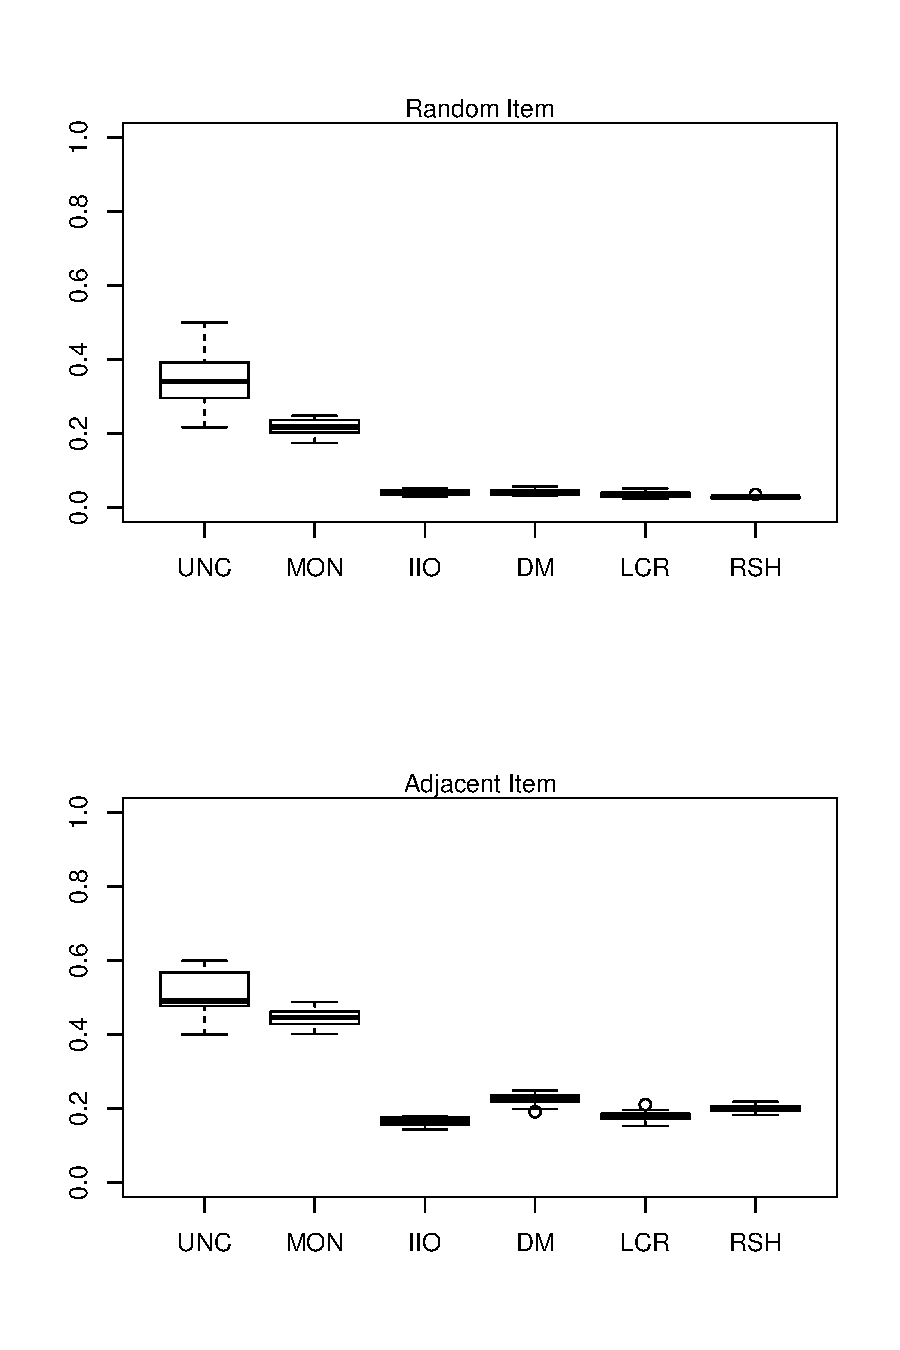
\includegraphics[height=\textheight]{./figs/boxplots}
\end{figure}


\subsection{Reconsidering double cancellation}
As described in \citeA{domingue2013}, checking for double cancellation is challenging due to the lack of order along the minor diagonals. Evidence presented in the below sections demonstrate that, in fact, there tends to be little difference between the checks with double cancellation, as implemented in \citeA{conjointchecks}, and a version that only requires both forms of single cancellation. To illustrate this point, data from \citeA<Table 2>{perline1979} is used.

\subsubsection{No advantage to double cancellation}
Figure \ref{single_example} compares mean violation rates for the adjacent and random checks when single and double cancellation are checked (denoted double) as opposed to only single cancellation (denoted single). For the random checks, there are essentially no differences. For the adjacent checks, there are small differences for items 3, 5, and 7. For these three, the addition of the double cancellation check adds a small amount of stringency. This is perhaps rather surprising. The next section is an attempt to demonstrate why this is happening.\footnote{At present, I'm addressing this by looking at the methodology from my dissertatoin. Another way of framing this issue would be via simulation. Basically, with simulated data (where truth is known), how often does double cancellation even need to hold (how often is the precedent true)? This might be nice.}


\begin{figure}
\centering
\caption{Comparison of violation means for single and single+double cancellation checks.} \label{single_example}
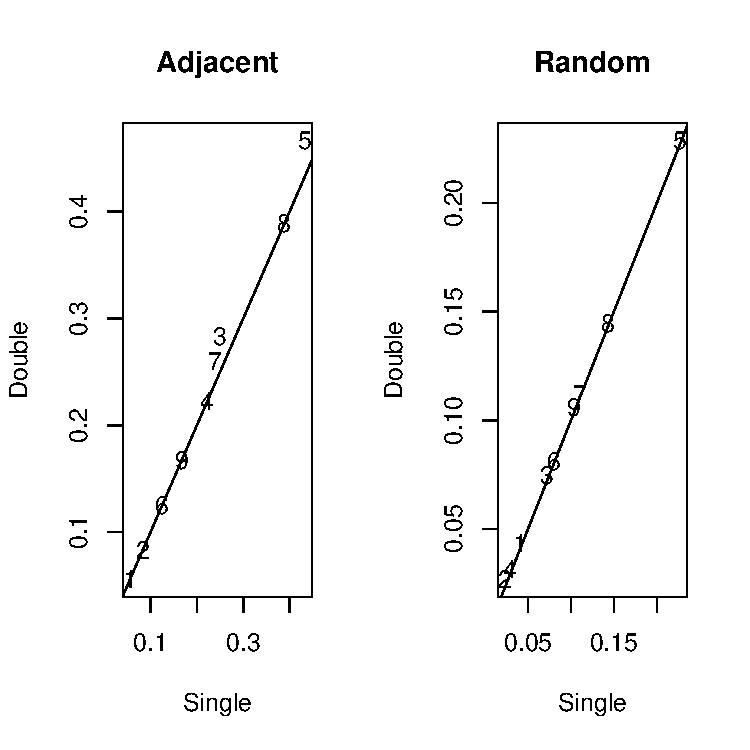
\includegraphics[width=\textwidth]{./figs/single_example}
\end{figure}

\subsubsection{The difficulty of checking for double cancellation}
To understand why double cancellation is such a fickle issue with empirical data, it will help to demonstrate via a few empirical examples. Let us begin with rows 3 through 5 of the \citeA{perline1979} data and items 2, 4, and 9. The empirical proportions are:
\[
\begin{array}{ccc}
0.15& 0.39& 0.67 \\
0.24 &0.40 &0.70 \\
 0.33& 0.51& 0.78 
\end{array}.
\]
This 3-matrix was chosen since it is seemingly (in terms of observed data, not true values) in compliance with one form of double cancellation. Focus on the $(1,3)$ element. Given the fact that $0.24<0.39$ and $0.51<0.70$, it should be (and is) the case that $0.33<0.67$. Let us monitor the nature of the checks as iterations of the Markov chain are accumulated. The basic fact is that the addition of double cancellation here is just not especially stringent. As an example, here are the updated values after the first 1000 iterations of the chain:
\[
\begin{array}{ccc}
0.14 &0.28& 0.62 \\
 0.23& 0.42& 0.65 \\
 0.31& 0.53& 0.86
\end{array}.
\]
In terms of the limits that make up the jumping distribution in the ``woven''\footnote{I'm introducing this term to deal with the fact that these chains are being updated simultaneously.} Metropolis-Hastings algorithm, the upper-right cell needs to be bigger than 0.28 because of single cancellation and, given that the precedent of double cancellation seems to hold, larger than 0.31. This difference is very slight. Checking for only single cancellation is effectively no different.

If we now look at rows 4 through 6 and columns 4 through 6, we observe a much messier scenario:
\[
\begin{array}{ccc}
 0.40& 0.52& 0.51 \\
 0.51& 0.73& 0.68 \\
 0.58& 0.95& 0.91
\end{array}.
\]
Here we have an example where a consequent of double cancellation regarding the order of the $(1,3)$ and $(3,1)$ cells is unneccessary since there is no consistent ordering regarding the pairs $(1,2),(2,1)$ and $(2,3), (3,2)$. One final example will round out the demonstration. NOW FINISH WITH AN EXAMPLE WHERE  ORDERING OF THOSE PAIRS HOLDS BUT NOT THE CORNERS. THIS WOULD BE THE ONE CASE WHERE IT MATTERS. demonstrate perhaps that it does. 

For the data examined here, there are only 5 cases where 3-matrices formed from adjacent cells have empirical proporotions of correct responses that correspond to violations of double cancellation and none of these 3-matrices are violations in the sense described in \citeA{domingue2013}. An alternative way of understanding what is going on might be to compare double cancellation within simulated Rasch data. Let $S_1$ be the truth value of the statement $\theta_{2,1}>\theta_{1,2}$ and $S_2$ the truth value of the statement $\theta_{3,2}>\theta_{2,3}$. These are the statements that are involved in both forms of the interesting statement of double cancellation. Let $S_3$ be the truth value of $\theta_{3,1}>\theta_{1,3}$. Table \ref{dc.sim} tabulates these truth values from a DESCRIBE SIMULATION. Bold numbers in the table indicate violations. Note that there are no violations with the true probabilities from the Rasch model. This is to be expected given that the Rasch model is known to uphold the axioms of additive conjoint measurement. However, with the observed proportions, we observe violations in quite a large number of cases (proportionally) compared to other possibilities. The punchline is that double cancellation is ``violated'' with observed proportions even when the underlying probabilities are consistent with the axioms of ACM. Why is this? The next section is one potential answer.


\ctable[
pos=ht,
caption=Double Cancellation with simulated Rasch data,
label=dc.sim,
]{lcccc}{
}{
\toprule
&&&\multicolumn{2}{c}{$S_3$} \\ \cmidrule{4-5}
&$S_1$&$S_2$&TRUE&FALSE \\ \midrule                       
\multirow{4}*{True Probabilities}&TRUE&TRUE&      5&     {\bf 0} \\
&TRUE&FALSE      &       9   &12 \\
&FALSE&TRUE&      8&    8\\
&FALSE&FALSE&       {\bf 0}&    7 \\ \midrule
\multirow{4}*{Observed Proportions}&TRUE&TRUE&      9&    {\bf 9} \\
&TRUE&FALSE&       7&    5 \\
&FALSE&TRUE &      8&    3 \\
&FALSE&FALSE   &    {\bf 6}&    2 \\ \bottomrule
}



Perhaps make point that it is the unevenness of the items and ability levels that leads to the disorder on the minor diagonal.

\subsection{Effect of measurement error on violations?}
NOTE: I really like this section, but it needs to be tied in with the above (how does it affect violations)? I think we could also probably make a similar point with fit statistics. 

Consider a series of simulations based on 5000 respondents whose abilities are drawn from a normal distribution and three forms of a test: short, medium, and long. The short form, shown on the top of Figure \ref{noise}, consists of 20 items. Figure \ref{noise} displays the true score SD for all true scores whose simulated response strings yield a given sum score. For the short form, each sum score contains a set of indivuals the SD of whose true scores is fairly consistently equal to {\em or greater than} the SD of all the true scores. This is a different way of looking at measurement error. From this perspective, the sorting done by the test of the respondees into different ability groups is no greater than we would expect than if the respondees were just sorted randomly. The medium length test form, 50 items, has a true score SD for each sum score that is typically around 1/3 of the overall true score SD. The long form, 500 items, is too long to be practical for most applications but is considered as an example. For this form, the true score SD for each sum score is around 20\% of the overall true score SD.

\begin{figure}
\centering
\caption{SD in true scores as a function of observed sum scores.} \label{noise}
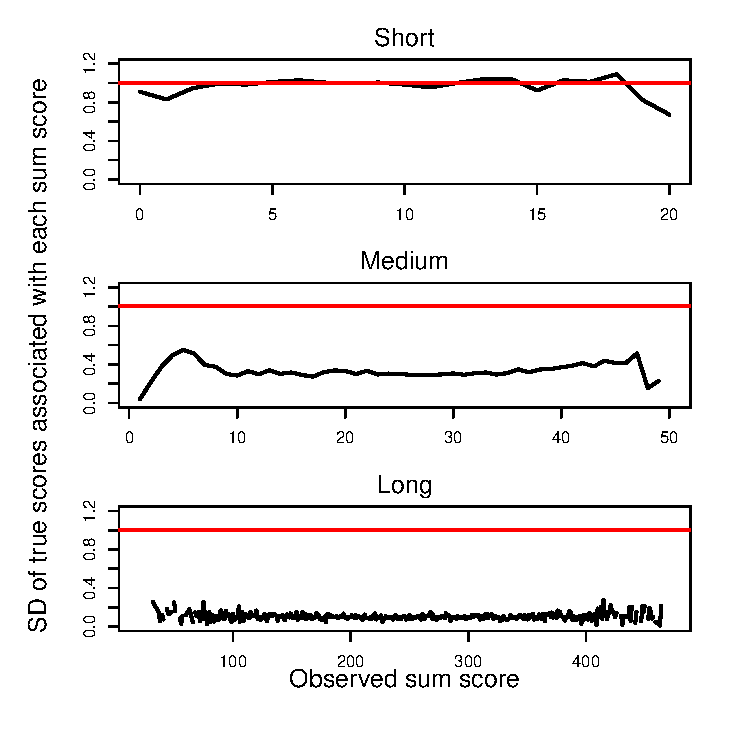
\includegraphics[width=\textwidth]{./figs/noise}1
\end{figure}

\subsection{Scale Distortions}
In this section, I want to compare the LCR and RSH models using my ``difference matrix'' approach. I have no idea what we'll find, but I think it could be really cool.


\putbib{conjoint}

\end{document}
